%%%%%%%%%%%%%%%%%%%%%%%%%%%%%%%%%%%%%%%%%
% Beamer Presentation
% LaTeX Template
% Version 1.0 (10/11/12)
%
% This template has been downloaded from:
% http://www.LaTeXTemplates.com
%
% License:
% CC BY-NC-SA 3.0 (http://creativecommons.org/licenses/by-nc-sa/3.0/)
%
%%%%%%%%%%%%%%%%%%%%%%%%%%%%%%%%%%%%%%%%%

%----------------------------------------------------------------------------------------
%	PACKAGES AND THEMES
%----------------------------------------------------------------------------------------

\documentclass{beamer}

\mode<presentation> {
\usepackage{listings}

% The Beamer class comes with a number of default slide themes
% which change the colors and layouts of slides. Below this is a list
% of all the themes, uncomment each in turn to see what they look like.

%\usetheme{default}
%\usetheme{AnnArbor}
%\usetheme{Antibes}
%\usetheme{Bergen}
%\usetheme{Berkeley}
%\usetheme{Berlin}
%\usetheme{Boadilla}
%\usetheme{CambridgeUS}
%\usetheme{Copenhagen}
%\usetheme{Darmstadt}
%\usetheme{Dresden}
%\usetheme{Frankfurt}
%\usetheme{Goettingen}
%\usetheme{Hannover}
%\usetheme{Ilmenau}
%\usetheme{JuanLesPins}
%\usetheme{Luebeck}
%\usetheme{Madrid}
%\usetheme{Malmoe}
%\usetheme{Marburg}
%\usetheme{Montpellier}
%\usetheme{PaloAlto}
%\usetheme{Pittsburgh}
%\usetheme{Rochester}
%\usetheme{Singapore}
%\usetheme{Szeged}
\usetheme{Warsaw}

% As well as themes, the Beamer class has a number of color themes
% for any slide theme. Uncomment each of these in turn to see how it
% changes the colors of your current slide theme.

%\usecolortheme{albatross}
\usecolortheme{beaver}
%\usecolortheme{beetle}
%\usecolortheme{crane}
%\usecolortheme{dolphin}
%\usecolortheme{dove}
%\usecolortheme{fly}
%\usecolortheme{lily}
%\usecolortheme{orchid}
%\usecolortheme{rose}
%\usecolortheme{seagull}
%\usecolortheme{seahorse}
%\usecolortheme{whale}
%\usecolortheme{wolverine}

%\setbeamertemplate{footline} % To remove the footer line in all slides uncomment this line
%\setbeamertemplate{footline}[page number] % To replace the footer line in all slides with a simple slide count uncomment this line

%\setbeamertemplate{navigation symbols}{} % To remove the navigation symbols from the bottom of all slides uncomment this line
}

\usepackage{graphicx} % Allows including images
\usepackage{booktabs} % Allows the use of \toprule, \midrule and \bottomrule in tables

%----------------------------------------------------------------------------------------
%	TITLE PAGE
%----------------------------------------------------------------------------------------

\title[Algebraic Multigrid]{Iterative Solvers - Algebraic Multigrid} % The short title appears at the bottom of every slide, the full title is only on the title page

\author{Bernd Schwarzenbacher, Daniel Herold} % Your name
\institute[TU Wien] % Your institution as it will appear on the bottom of every slide, may be shorthand to save space
{Technical University of Vienna \\ % Your institution for the title page
\medskip
%\textit{john@smith.com} % Your email address
}
\date{\today} % Date, can be changed to a custom date

\begin{document}

\begin{frame}
\titlepage % Print the title page as the first slide
\end{frame}

%\begin{frame}
%\frametitle{Overview} % Table of contents slide, comment this block out to remove it
%\tableofcontents % Throughout your presentation, if you choose to use \section{} and \subsection{} commands, these will automatically be printed on this slide as an overview of your presentation
%\end{frame}

%------------------------------------------------------------------------------
%	PRESENTATION SLIDES
%------------------------------------------------------------------------------

%------------------------------------------------
%------------------------------------------------

\begin{frame}
\frametitle{Iterative Solvers}
fixed-point equation:
$$b = Ax \iff x = x + C^{-1} (b-Ax)$$
\begin{block}{Richardson Iteration}
start value $x_{0}$ \\
for $j = 0, 1, 2, \dots$ \\
\quad $x^{j+1} = x^{j} + C^{-1} (b - Ax^{j})$
\end{block}
\end{frame}

\begin{frame}
\frametitle{Preconditioning}
\begin{block}{Richardson Iteration}
$x^{new} = x^{old} + C^{-1} (b - Ax^{old})$
\end{block}
$C \dots$ preconditioner:
\begin{itemize}
  \item cheap matrix-vector multiplikation with $C^{-1}$
  \item good approximation of $A$
\end{itemize}
\end{frame}

\begin{frame}
\frametitle{Jacobi Preconditioner}
\begin{block}{Richardson Iteration}
$x^{new} = x^{old} + C^{-1} (b - Ax^{old})$
\end{block}
$$C = diag(A)$$
$$x_j^{new} = x_j^{old} + \frac{1}{A_{jj}} \left(b_{j} -
\sum_{k=1}^{n} A_{jk} x_k^{old}\right)$$
\end{frame}

\begin{frame}
\frametitle{Gau\ss-Seidel Preconditioner}
\begin{block}{Richardson Iteration}
$x^{new} = x^{old} + C^{-1} (b - Ax^{old})$
\end{block}
$$C = L + diag(A)$$
$$x_j^{new} = x_j^{old} + \frac{1}{A_{jj}} \left(b_{j} - \sum_{k=1}^{j-1} A_{jk}
x_k^{new} - \sum_{k=j}^{n} A_{jk} x_k^{old}\right)$$
\end{frame}

\begin{frame}
\frametitle{Multigrid Preconditioner}
$$x_{new} = x_{old} + P (P^{T} A P)^{-1} P^{T} (b - A x_{old})$$
$$P =
\begin{pmatrix}
  1 & 0 & 0 & 0 \\
  1 & 0 & 0 & 0 \\
  0 & 1 & 0 & 0 \\
  0 & 1 & 0 & 0 \\
  0 & 0 & 1 & 0 \\
  0 & 0 & 0 & 1 \\
  0 & 0 & 0 & 1 \\
  0 & 0 & 0 & 1 \\
\end{pmatrix}
$$
$P \dots$ prolongation matrix
\end{frame}

\begin{frame}
\frametitle{AMG - Algebraic Multigrid}
\begin{itemize}
  \item combine Multigrid and Gau\ss-Seidel preconditioner
  \item direct solver on coarsest level
  \item algebraic - artificial coarsening without information of mesh
\end{itemize}
\end{frame}

\begin{frame}
\frametitle{AMG - Parallelization}
\begin{itemize}
  \item Multigrid: transposed matrix-vector multiplication
    $$P^{T} (b-Ax^{old})$$
  \item Gau\ss-Seidel: \\ $$\frac{1}{A_{jj}} \left(b_{j} - \sum_{k=1}^{j-1} A_{jk}
x_k^{new} - \sum_{k=j}^{n} A_{jk} x_k^{old}\right)$$
\end{itemize}
\end{frame}

%-----------------------------------------------------------------------
\defverbatim[colored]\codeA{
\begin{lstlisting}[language=C++,basicstyle=\ttfamily,keywordstyle=\color{blue}]
for (int j = firsti[k]; j < lasti[k]; ++j)
      {...}

\end{lstlisting}
}

\begin{frame}
\frametitle{Sparse Matrices}
\begin{itemize}
\item internal storage: ccs-format
\item usage:
\begin{block}{indexing | for-loop}
\codeA
\end{block}
\end{itemize}
\end{frame}


\defverbatim[colored]\codeB{
\begin{lstlisting}[language=C++,basicstyle=\ttfamily,keywordstyle=\color{blue}]
    for (int i = 0; i < this->Height(); ++i)
    {
      int first = firsti [i];
      int last  = firsti [i+1];

      for (int j = first; j < last; ++j)
      {
        y(colnr[j]) += data[j] * x(i);
      }
    }
\end{lstlisting}
}

\begin{frame}
\frametitle{Transposed Matrix-Vector Multiplication}
problem: $A^T\cdot x=y$
\begin{block}{code section}
\codeB
\end{block}
\end{frame}

\defverbatim[colored]\codeC{
\begin{lstlisting}[language=C++,basicstyle=\ttfamily,keywordstyle=\color{blue}]
   #pragma omp for schedule (dynamic, 100)
\end{lstlisting}
}

\begin{frame}
\frametitle{Transposed Matrix-Vector Multiplication}
\textbf{problem with parallelization:}
\begin{itemize}
\item row indexing is necessary
\item multiple writing entries per row
\end{itemize}

\textbf{possible solutions:}
\begin{itemize}
\item atomic section
\item atomic section with dynamic thread partitioning \codeC
\item atomic section with static thread separation
\end{itemize}
\end{frame}

\begin{frame}
\frametitle{Coloring}
other solution: \textbf{matrix coloring}
\begin{itemize}
\item some rows do not interfere
\item build groups of rows (colors)
\item parallelize each color
\item run loop through different colors sequentially
\end{itemize}
\end{frame}

\begin{frame}
\frametitle{Coloring}
problem: $A^T \cdot x= y$
(example)
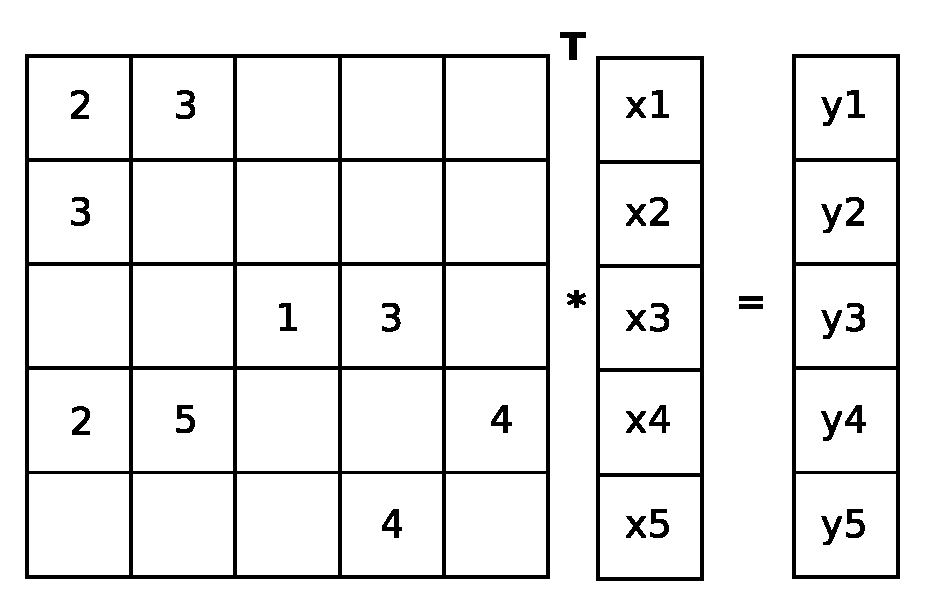
\includegraphics[width=0.8\linewidth]{graphic/coloringT1.eps}
\end{frame}

\begin{frame}
\frametitle{Coloring}
problem: $A^T \cdot x= y$
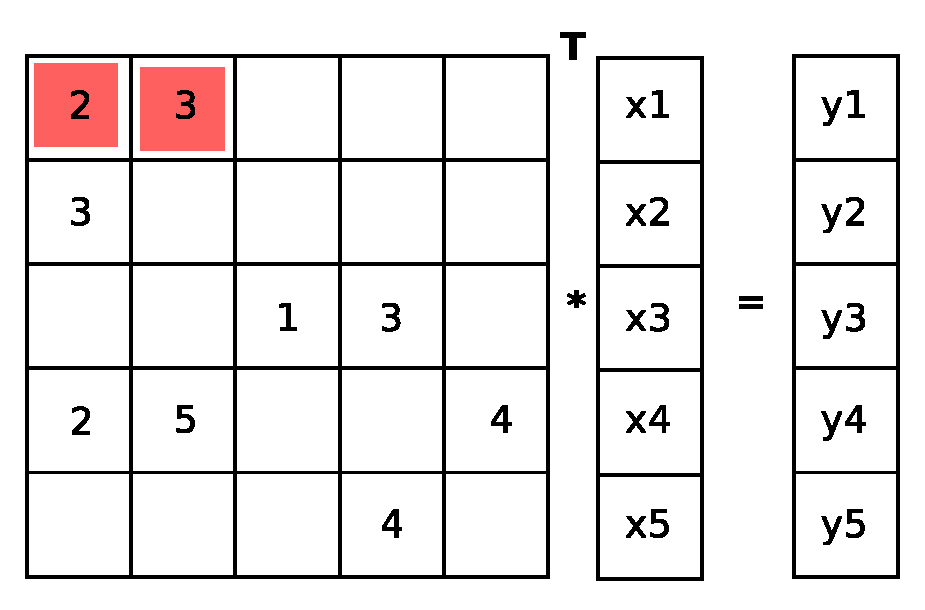
\includegraphics[width=0.8\linewidth]{graphic/coloringT2.eps}
\end{frame}

\begin{frame}
\frametitle{Coloring}
problem: $A^T \cdot x= y$
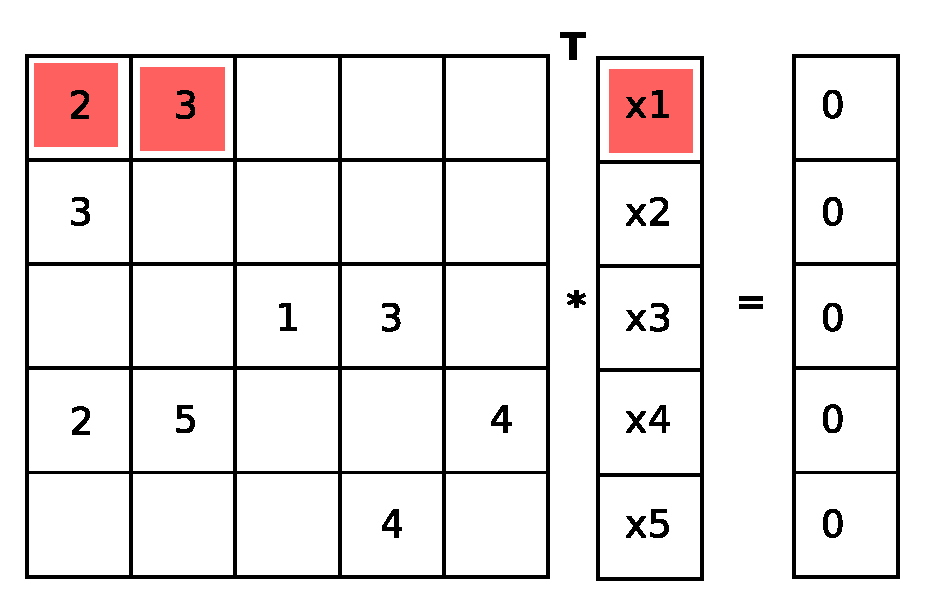
\includegraphics[width=0.8\linewidth]{graphic/coloringT3.eps}
\end{frame}


\begin{frame}
\frametitle{Coloring}
problem: $A^T \cdot x= y$
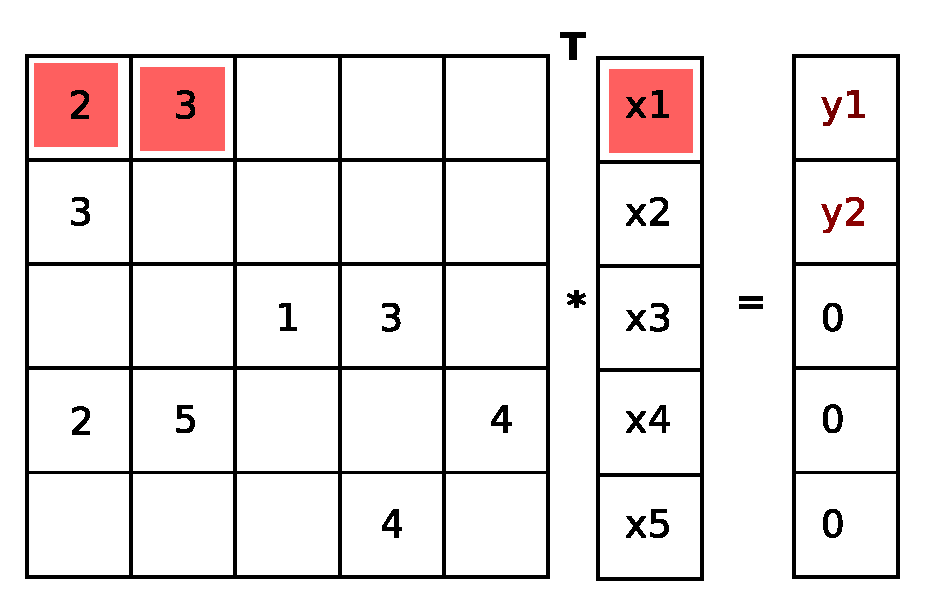
\includegraphics[width=0.8\linewidth]{graphic/coloringT4.eps}
\end{frame}

\begin{frame}
\frametitle{Coloring}
problem: $A^T \cdot x= y$
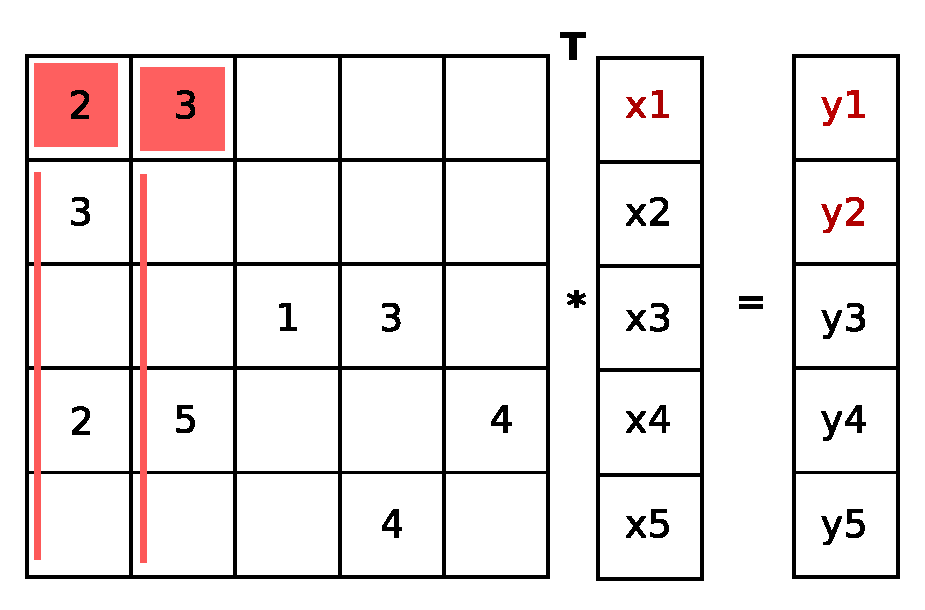
\includegraphics[width=0.8\linewidth]{graphic/coloringT5.eps}
\end{frame}

\begin{frame}
\frametitle{Coloring}
problem: $A^T \cdot x= y$
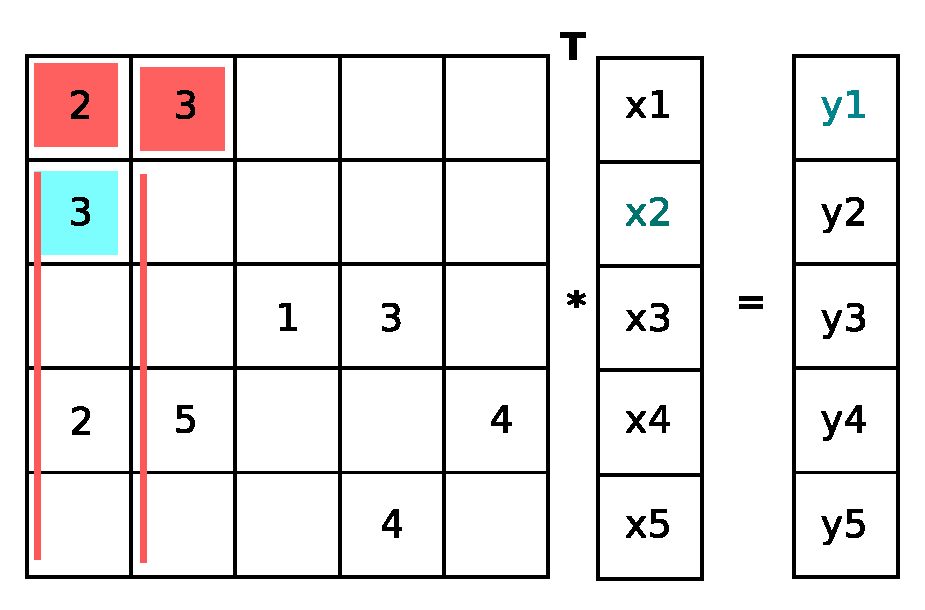
\includegraphics[width=0.8\linewidth]{graphic/coloringT6.eps}
\end{frame}

\begin{frame}
\frametitle{Coloring}
problem: $A^T \cdot x= y$
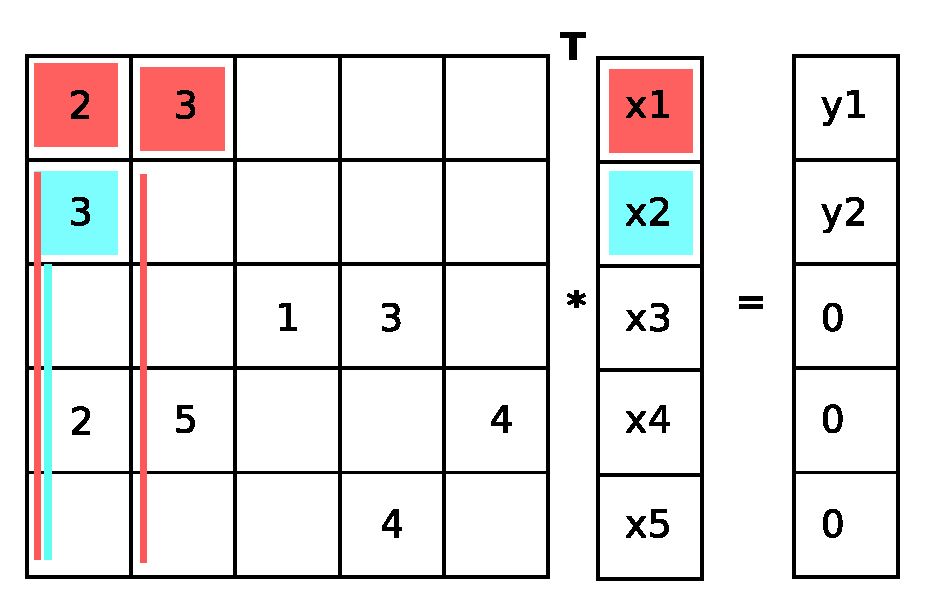
\includegraphics[width=0.8\linewidth]{graphic/coloringT7.eps}
\end{frame}

\begin{frame}
\frametitle{Coloring}
problem: $A^T \cdot x= y$
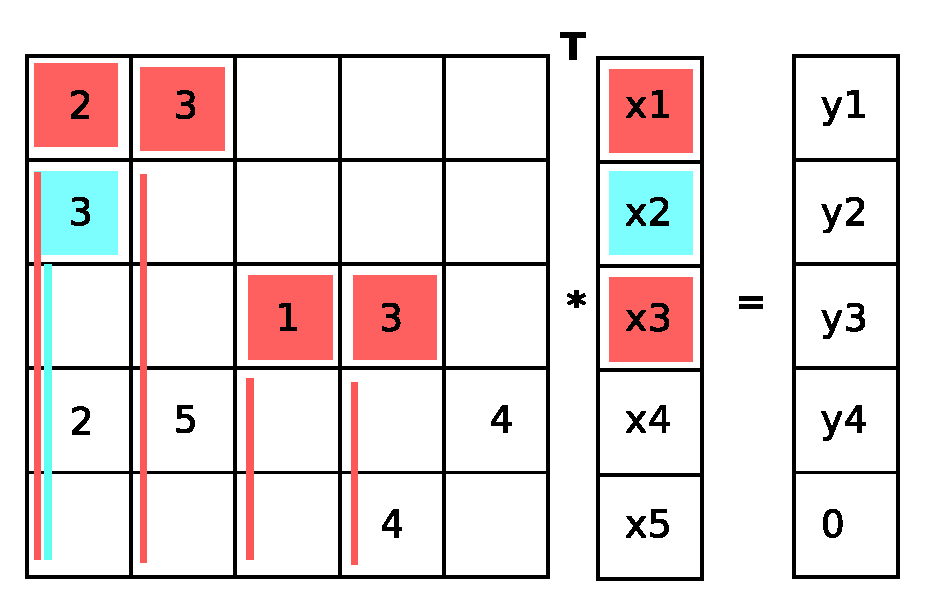
\includegraphics[width=0.8\linewidth]{graphic/coloringT8.eps}
\end{frame}

\begin{frame}
\frametitle{Coloring}
problem: $A^T \cdot x= y$
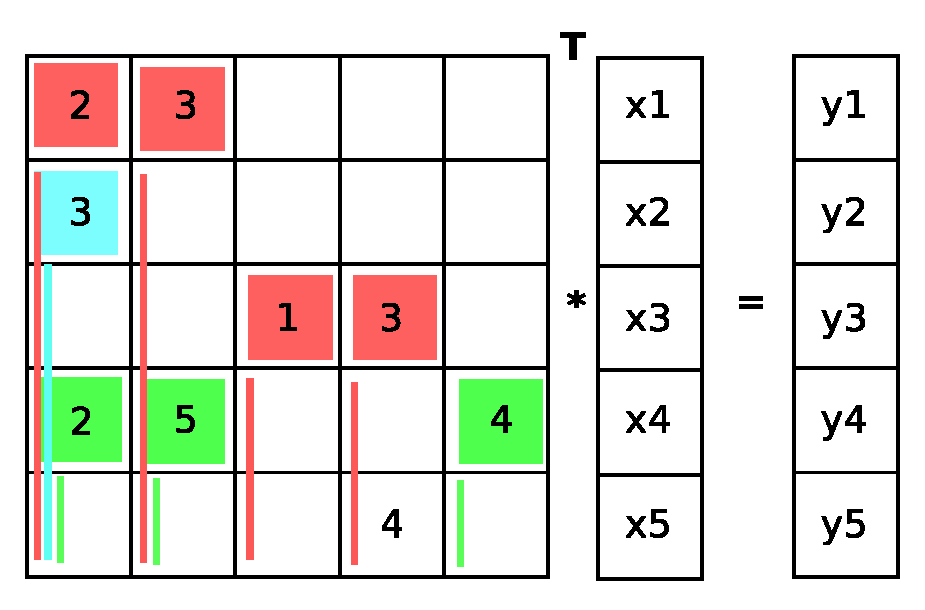
\includegraphics[width=0.8\linewidth]{graphic/coloringT9.eps}
\end{frame}

\begin{frame}
\frametitle{Coloring}
problem: $A^T \cdot x= y$
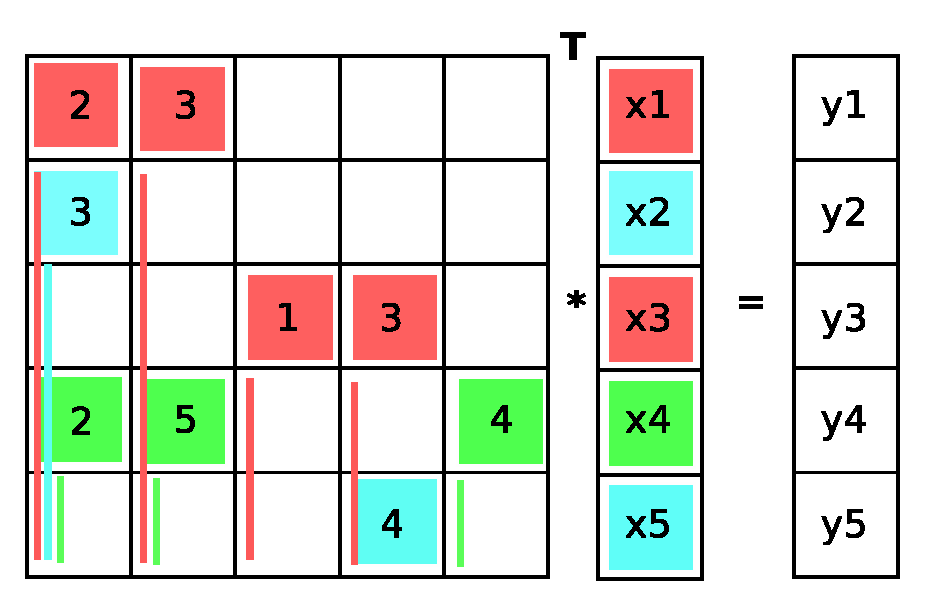
\includegraphics[width=0.8\linewidth]{graphic/coloringT10.eps}
\end{frame}

\begin{frame}
\frametitle{Coloring}
\textbf{disadvantage:}
\begin{itemize}
\item coloring has to be done separately
\end{itemize}

\textbf{advantages:}
\begin{itemize}
\item row indexing
\item no atomic sections
\item calculated coloring could be used often
\end{itemize}
\end{frame}

\begin{frame}
\frametitle{Time Measurement}
\begin{table}
\begin{tabular}{l l l}
\toprule
\textbf{method} & \textbf{time} & \textbf{flops}\\
\midrule
sequential & 2.55 sec & 480 MFlops \\
atomic & 1.25 sec & 980 MFlops \\
dynamic & 2.93 sec & 420 MFlops \\
balancing & 1.18 sec & 1040 MFlops \\
coloring\footnote{about 500 colors, 17 sec} & 1.75 sec & 700 MFlops \\
\bottomrule
\end{tabular}
\caption{matrix dimension: $29\cdot 10^6$, non-zero entries: $1.2\cdot 10^9$}
\end{table}
\end{frame}
%----------------------------------------------------------
%---------------------------------------------------------

\begin{frame}
\frametitle{Gau\ss-Seidel Preconditioner}
\begin{block}{Richardson Iteration}
$x^{new} = x^{old} + C^{-1} (b - Ax^{old})$
\end{block}
$$C = L + diag(A)$$
$$x_j^{new} = x_j^{old} + \frac{1}{A_{jj}} \left(b_{j} - \sum_{k=1}^{j-1} A_{jk}
x_k^{new} - \sum_{k=j}^{n} A_{jk} x_k^{old}\right)$$

\end{frame}

\begin{frame}
\frametitle{Gau\ss-Seidel Preconditioner}

\textbf{parallelization:}
\begin{itemize}
\item calculation of $x_j^{new}$ uses old and new entries
\item $x_j^{new}$ overwrites $x_j^{old}$
\item \textbf{problem:} some threads will write while others read
\item \textbf{problem:} each call of method causes different dependencies of $x_j$
\item \textbf{solution:}
coloring
\end{itemize}


$$ x_j^{new} = x_{old} + \frac{1}{A_{jj}} \left(b_{j} - \sum_{k \in K^{new}}A_{jk}
 x_k^{new} - \sum_{k \in K^{old}}A_{jk} x_k^{old}\right)$$
$K^{new}$ ... calculated indices of $x$;
$K^{old}$ ... old indices of $x$
\end{frame}

\begin{frame}
\frametitle{Coloring}
$ x_j^{new} = x_{old} + \frac{1}{A_{jj}} \left(b_{j} - \sum_{k \in K^{new}}A_{jk}
 x_k^{new} - \sum_{k \in K^{old}}A_{jk} x_k^{old}\right)$
example:
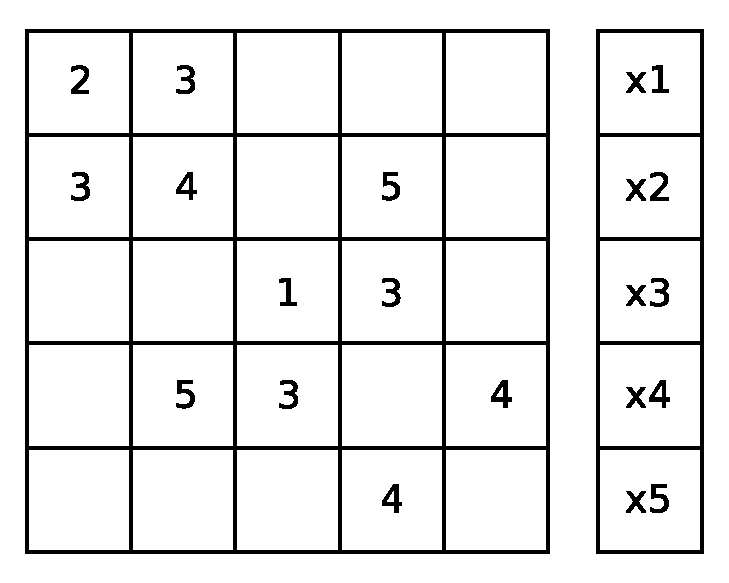
\includegraphics[width=0.8\linewidth]{graphic/coloringGS1.eps}
\end{frame}

\begin{frame}
\frametitle{Coloring}
$ x_j^{new} = x_{old} + \frac{1}{A_{jj}} \left(b_{j} - \sum_{k \in K^{new}}A_{jk}
 x_k^{new} - \sum_{k \in K^{old}}A_{jk} x_k^{old}\right)$
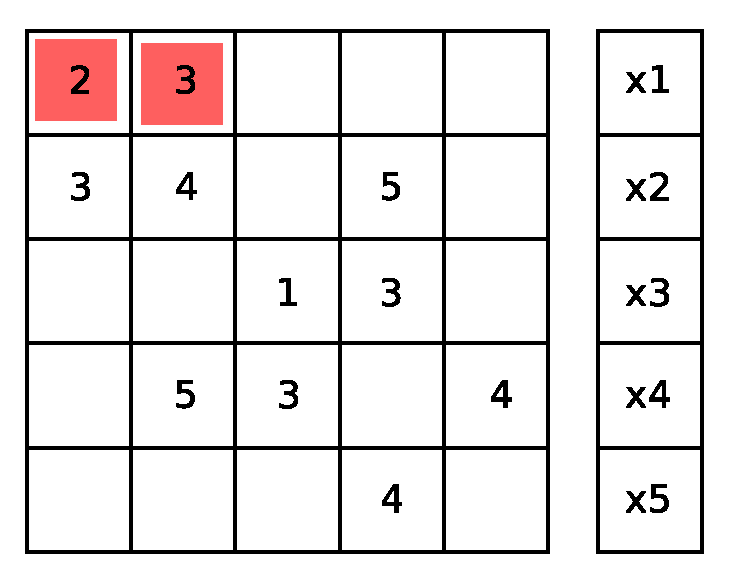
\includegraphics[width=0.8\linewidth]{graphic/coloringGS2.eps}
\end{frame}

\begin{frame}
\frametitle{Coloring}
$ x_j^{new} = x_{old} + \frac{1}{A_{jj}} \left(b_{j} - \sum_{k \in K^{new}}A_{jk}
 x_k^{new} - \sum_{k \in K^{old}}A_{jk} x_k^{old}\right)$
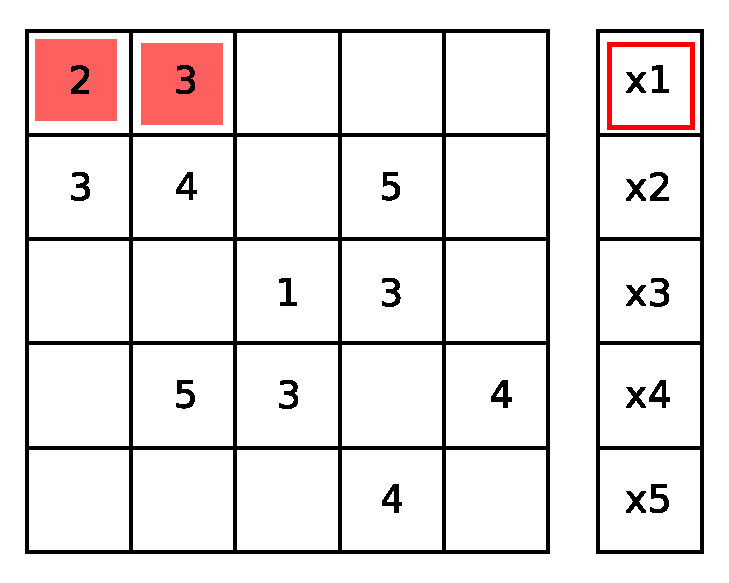
\includegraphics[width=0.8\linewidth]{graphic/coloringGS3.eps}
\end{frame}

\begin{frame}
\frametitle{Coloring}
$ x_j^{new} = x_{old} + \frac{1}{A_{jj}} \left(b_{j} - \sum_{k \in K^{new}}A_{jk}
 x_k^{new} - \sum_{k \in K^{old}}A_{jk} x_k^{old}\right)$
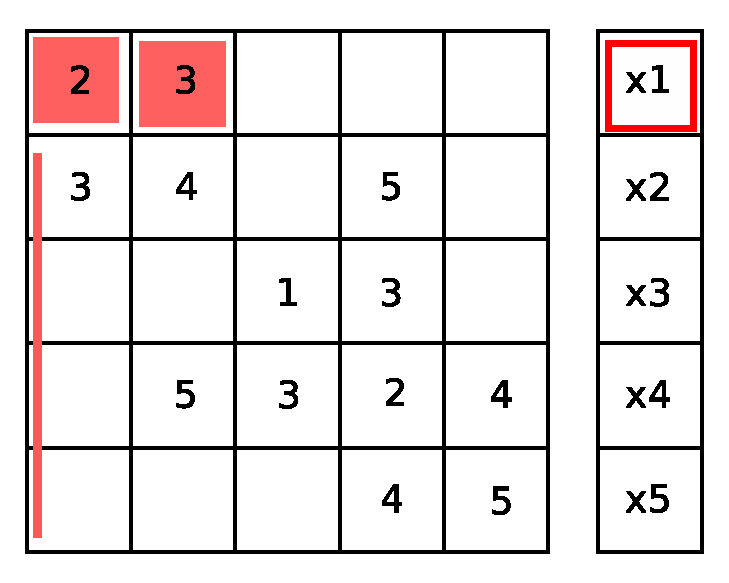
\includegraphics[width=0.8\linewidth]{graphic/coloringGS4.eps}
\end{frame}

\begin{frame}
\frametitle{Coloring}
$ x_j^{new} = x_{old} + \frac{1}{A_{jj}} \left(b_{j} - \sum_{k \in K^{new}}A_{jk}
 x_k^{new} - \sum_{k \in K^{old}}A_{jk} x_k^{old}\right)$
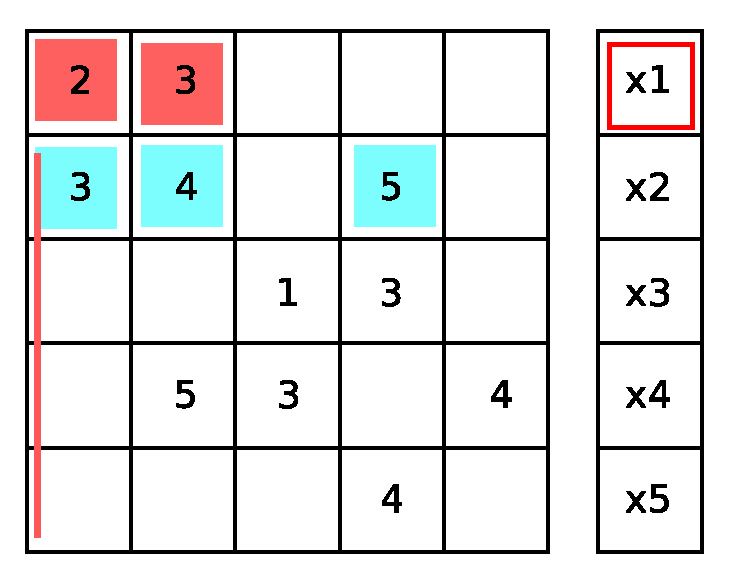
\includegraphics[width=0.8\linewidth]{graphic/coloringGS5.eps}
\end{frame}

\begin{frame}
\frametitle{Coloring}
$ x_j^{new} = x_{old} + \frac{1}{A_{jj}} \left(b_{j} - \sum_{k \in K^{new}}A_{jk}
 x_k^{new} - \sum_{k \in K^{old}}A_{jk} x_k^{old}\right)$
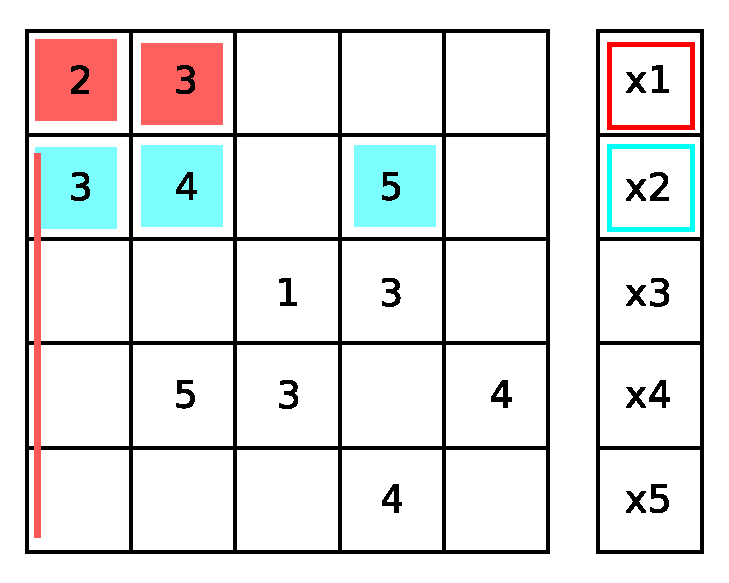
\includegraphics[width=0.8\linewidth]{graphic/coloringGS6.eps}
\end{frame}

\begin{frame}
\frametitle{Coloring}
$ x_j^{new} = x_{old} + \frac{1}{A_{jj}} \left(b_{j} - \sum_{k \in K^{new}}A_{jk}
 x_k^{new} - \sum_{k \in K^{old}}A_{jk} x_k^{old}\right)$
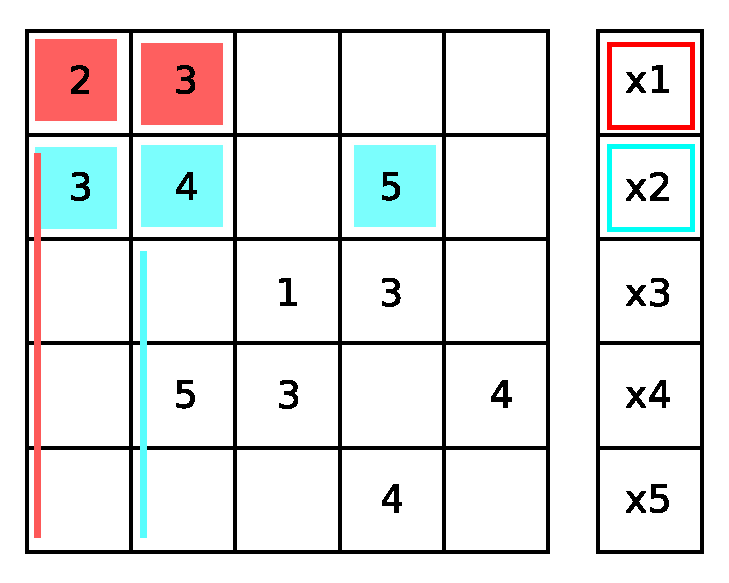
\includegraphics[width=0.8\linewidth]{graphic/coloringGS7.eps}
\end{frame}

\begin{frame}
\frametitle{Coloring}
$ x_j^{new} = x_{old} + \frac{1}{A_{jj}} \left(b_{j} - \sum_{k \in K^{new}}A_{jk}
 x_k^{new} - \sum_{k \in K^{old}}A_{jk} x_k^{old}\right)$
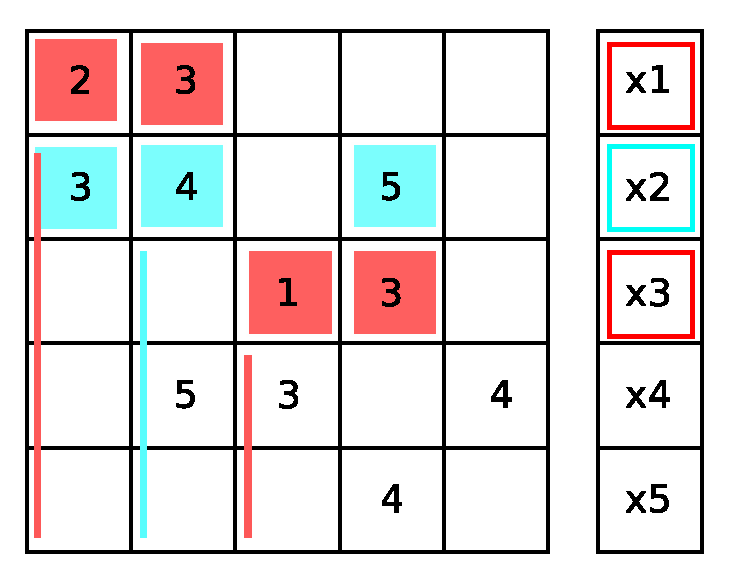
\includegraphics[width=0.8\linewidth]{graphic/coloringGS8.eps}
\end{frame}

\begin{frame}
\frametitle{Coloring}
$ x_j^{new} = x_{old} + \frac{1}{A_{jj}} \left(b_{j} - \sum_{k \in K^{new}}A_{jk}
 x_k^{new} - \sum_{k \in K^{old}}A_{jk} x_k^{old}\right)$
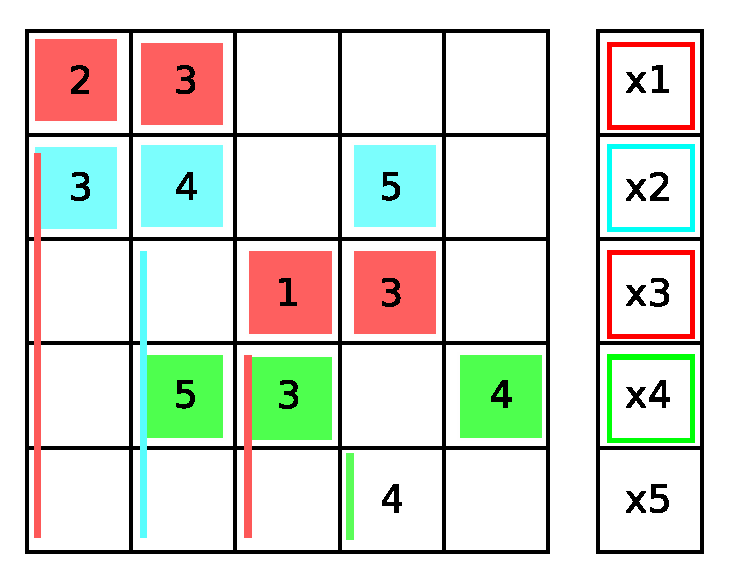
\includegraphics[width=0.8\linewidth]{graphic/coloringGS9.eps}
\end{frame}

\begin{frame}
\frametitle{Coloring}
$ x_j^{new} = x_{old} + \frac{1}{A_{jj}} \left(b_{j} - \sum_{k \in K^{new}}A_{jk}
 x_k^{new} - \sum_{k \in K^{old}}A_{jk} x_k^{old}\right)$
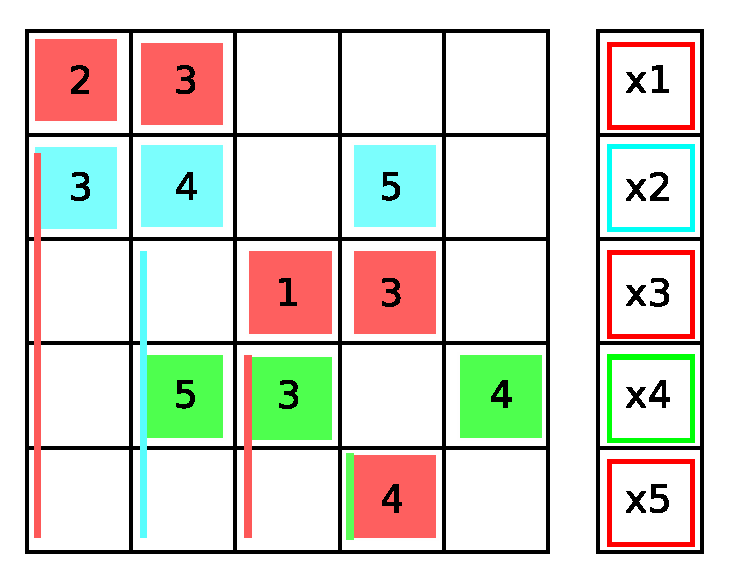
\includegraphics[width=0.8\linewidth]{graphic/coloringGS10.eps}
\end{frame}

\begin{frame}
$ x_j^{new} = x_{old} + \frac{1}{A_{jj}} \left(b_{j} - \sum_{k \in K^{new}}A_{jk}
 x_k^{new} - \sum_{k \in K^{old}}A_{jk} x_k^{old}\right)$
\frametitle{Coloring}
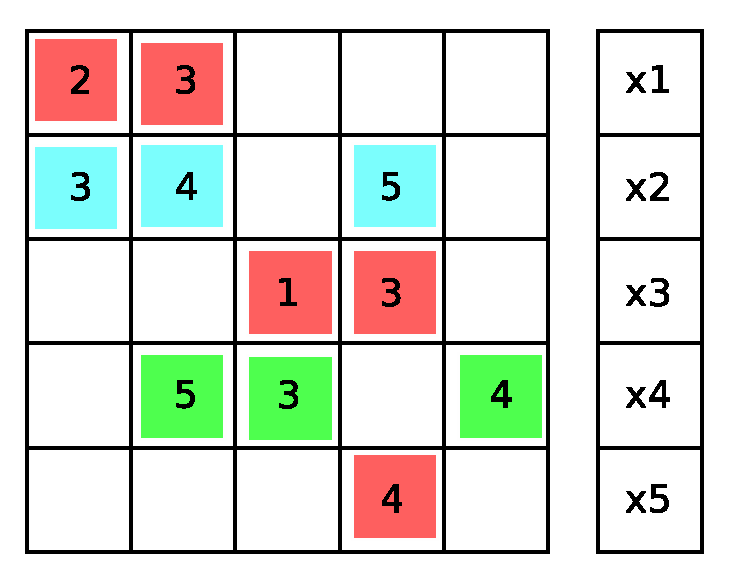
\includegraphics[width=0.8\linewidth]{graphic/coloringGS11.eps}
\end{frame}

\begin{frame}
\frametitle{Coloring}
$ x_j^{new} = x_{old} + \frac{1}{A_{jj}} \left(b_{j} - \sum_{k \in K^{new}}A_{jk}
 x_k^{new} - \sum_{k \in K^{old}}A_{jk} x_k^{old}\right)$
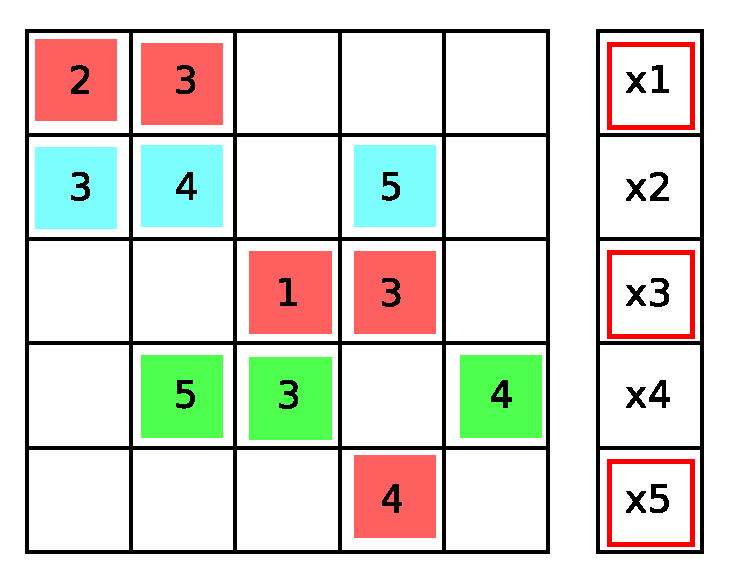
\includegraphics[width=0.8\linewidth]{graphic/coloringGS12.eps}
\end{frame}

\begin{frame}
\frametitle{Coloring}
$ x_j^{new} = x_{old} + \frac{1}{A_{jj}} \left(b_{j} - \sum_{k \in K^{new}}A_{jk}
 x_k^{new} - \sum_{k \in K^{old}}A_{jk} x_k^{old}\right)$
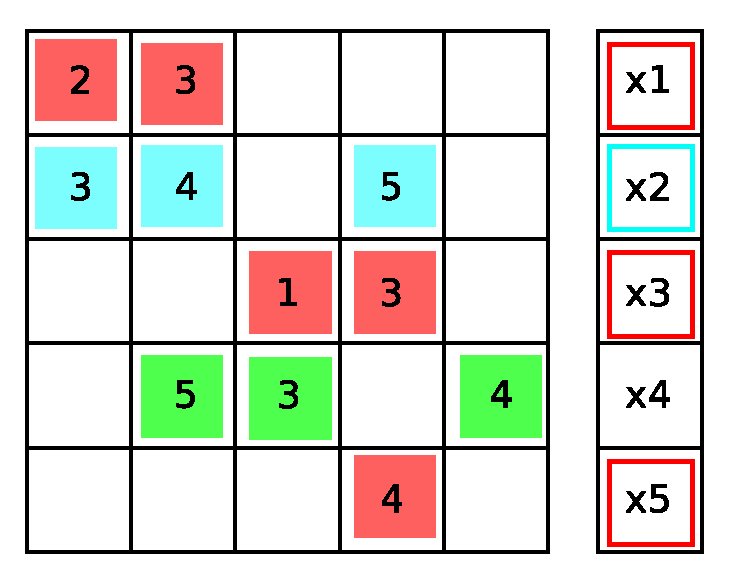
\includegraphics[width=0.8\linewidth]{graphic/coloringGS13.eps}
\end{frame}

\begin{frame}
\frametitle{Coloring}
$ x_j^{new} = x_{old} + \frac{1}{A_{jj}} \left(b_{j} - \sum_{k \in K^{new}}A_{jk}
 x_k^{new} - \sum_{k \in K^{old}}A_{jk} x_k^{old}\right)$
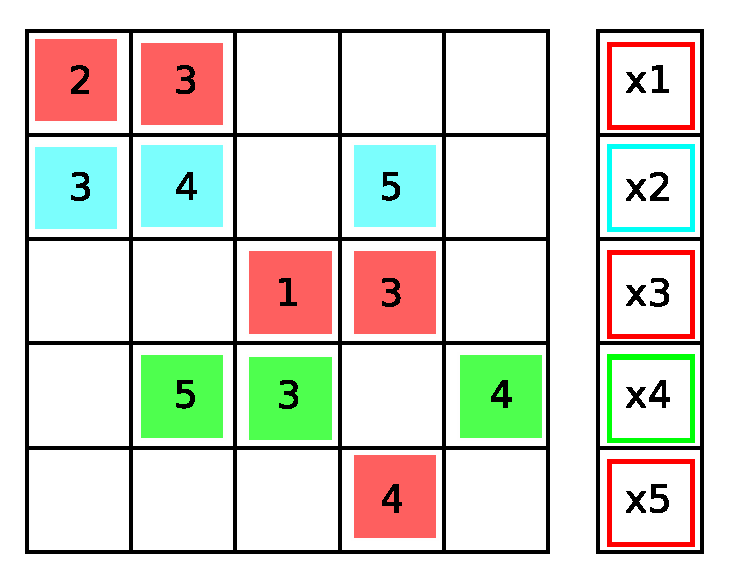
\includegraphics[width=0.8\linewidth]{graphic/coloringGS14.eps}
\end{frame}
%--------------------------------------------------------------

\begin{frame}
\frametitle{Gau\ss-Seidel - Coloring}
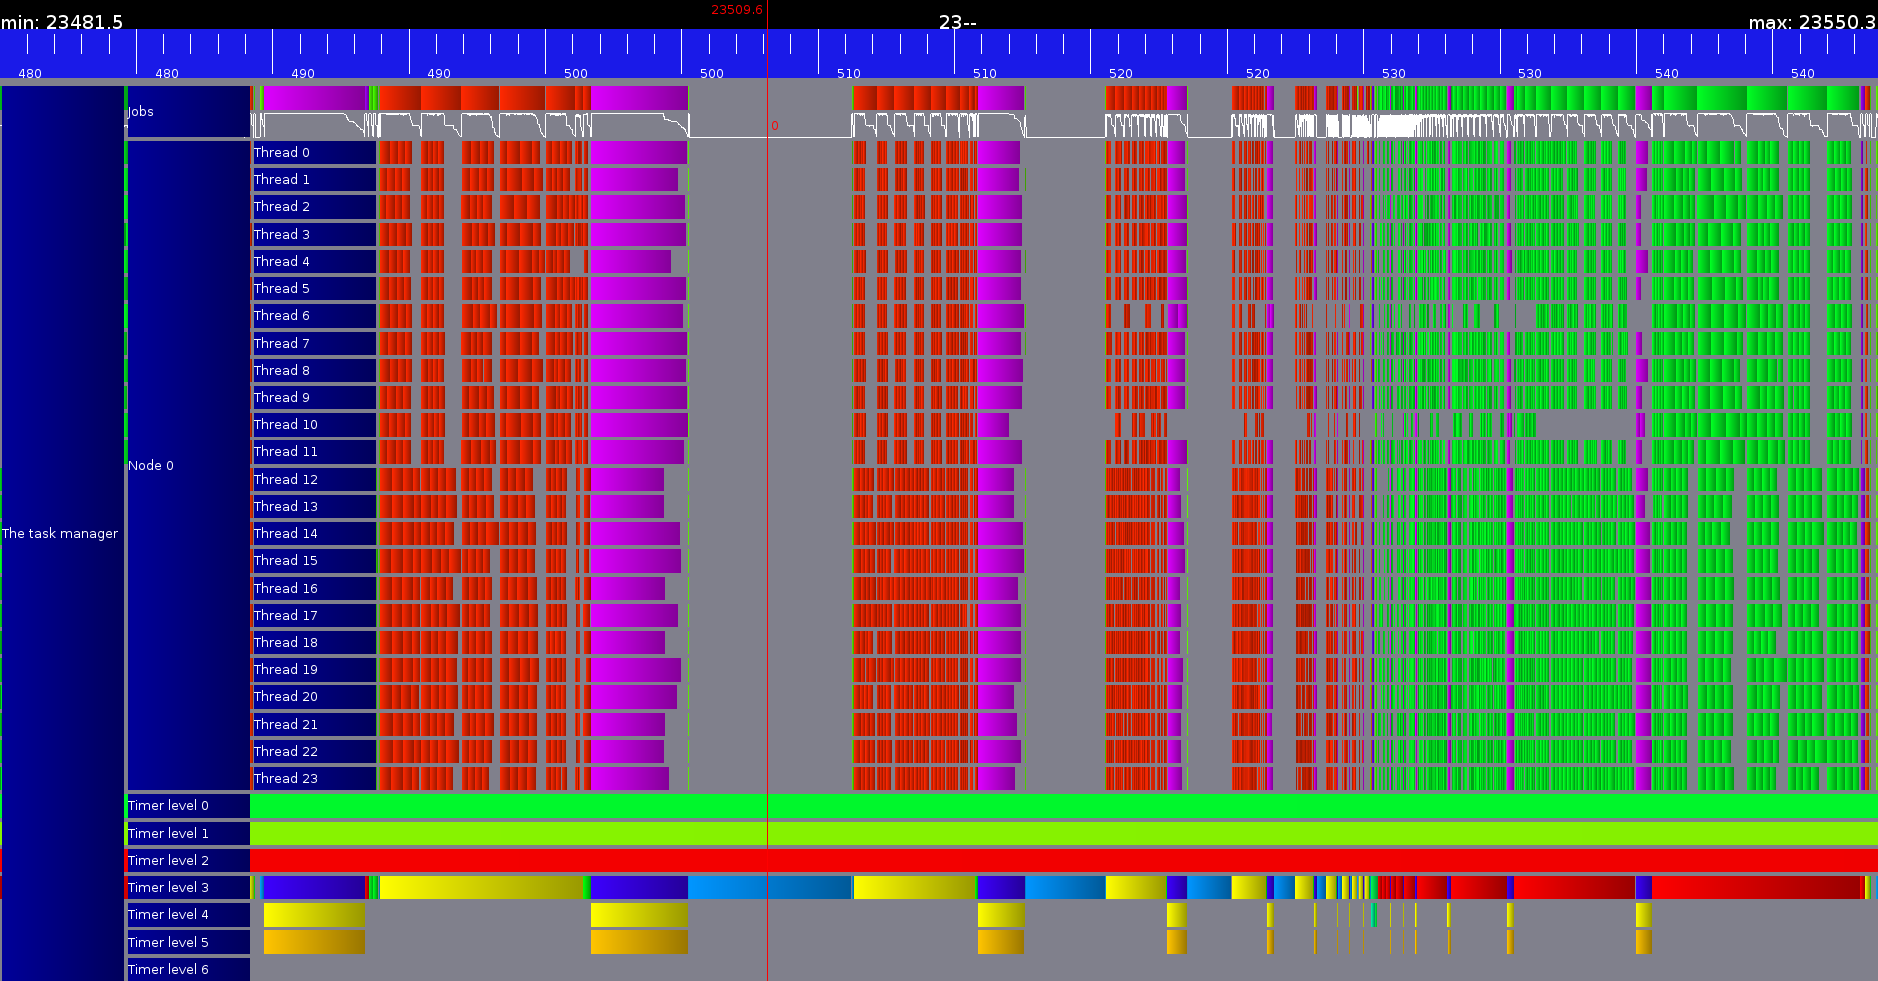
\includegraphics[width=1\linewidth]{undistributed_coloring_gs.png}
\end{frame}

\begin{frame}
\frametitle{Gau\ss-Seidel - Distributed Coloring \& Balancing}
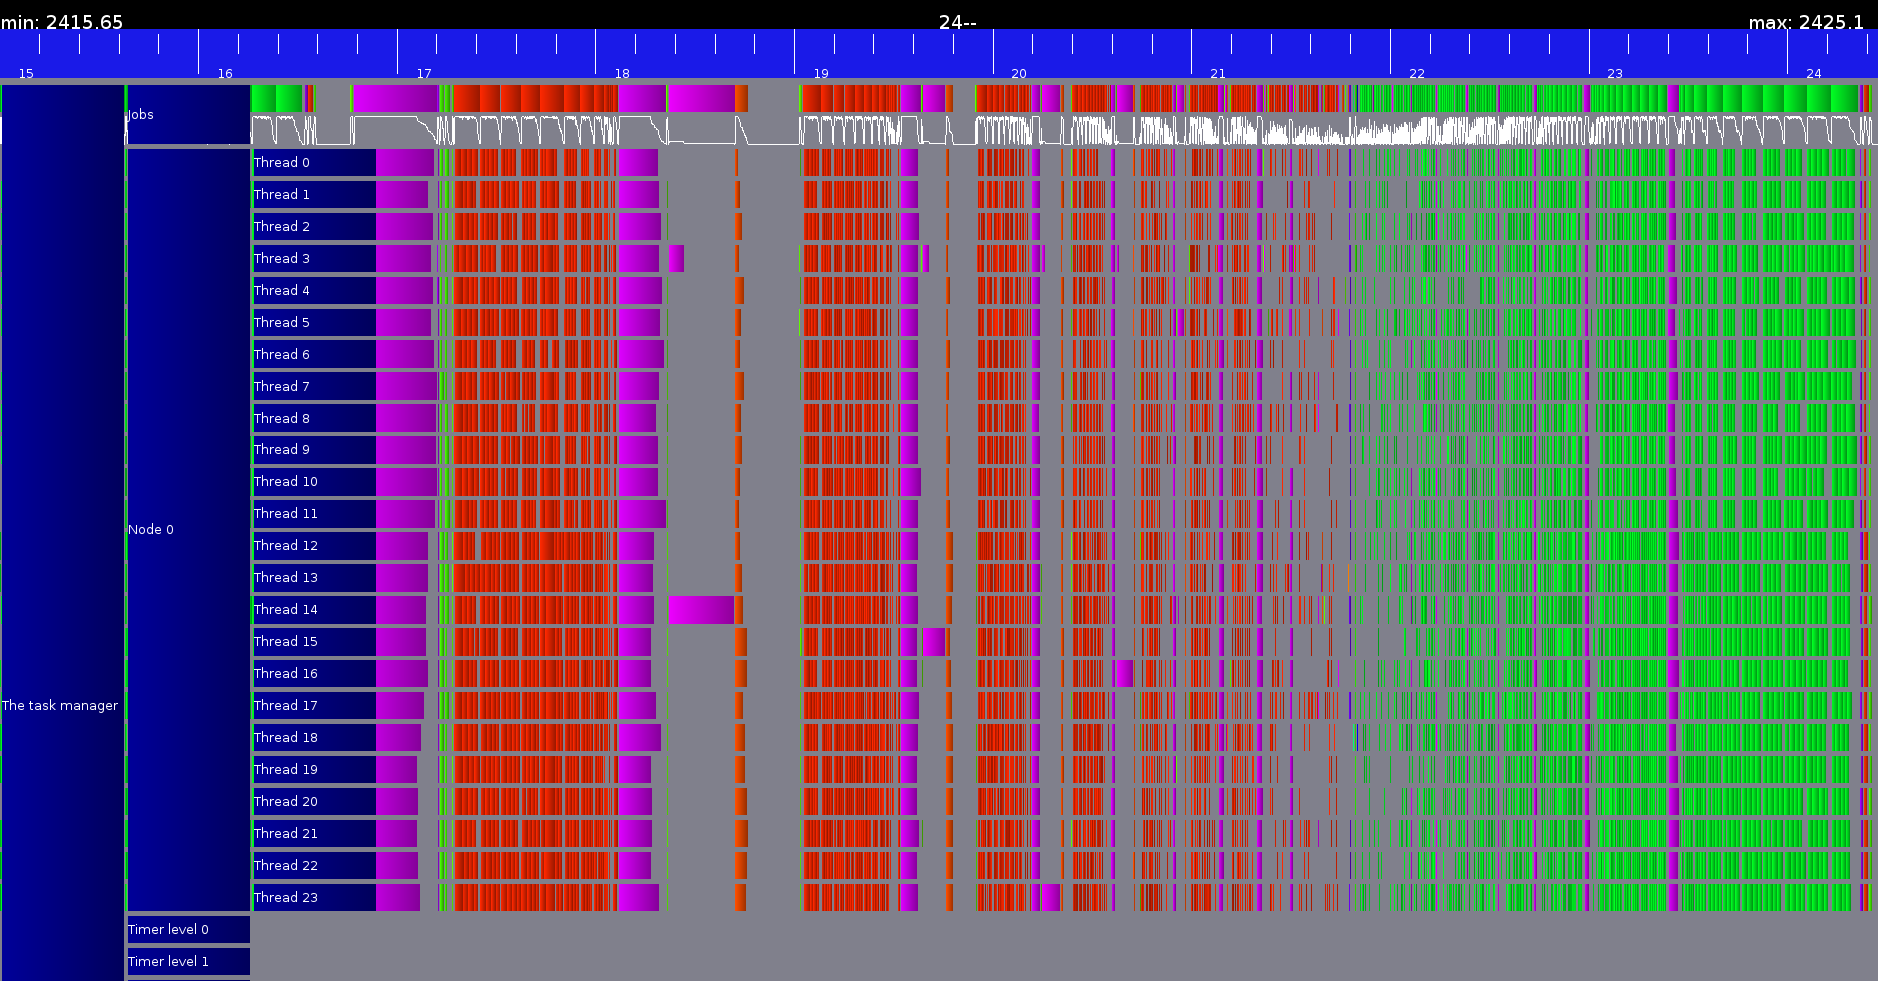
\includegraphics[width=1\linewidth]{one_iteration.png}
\end{frame}

\begin{frame}
\frametitle{CG - Iterations}
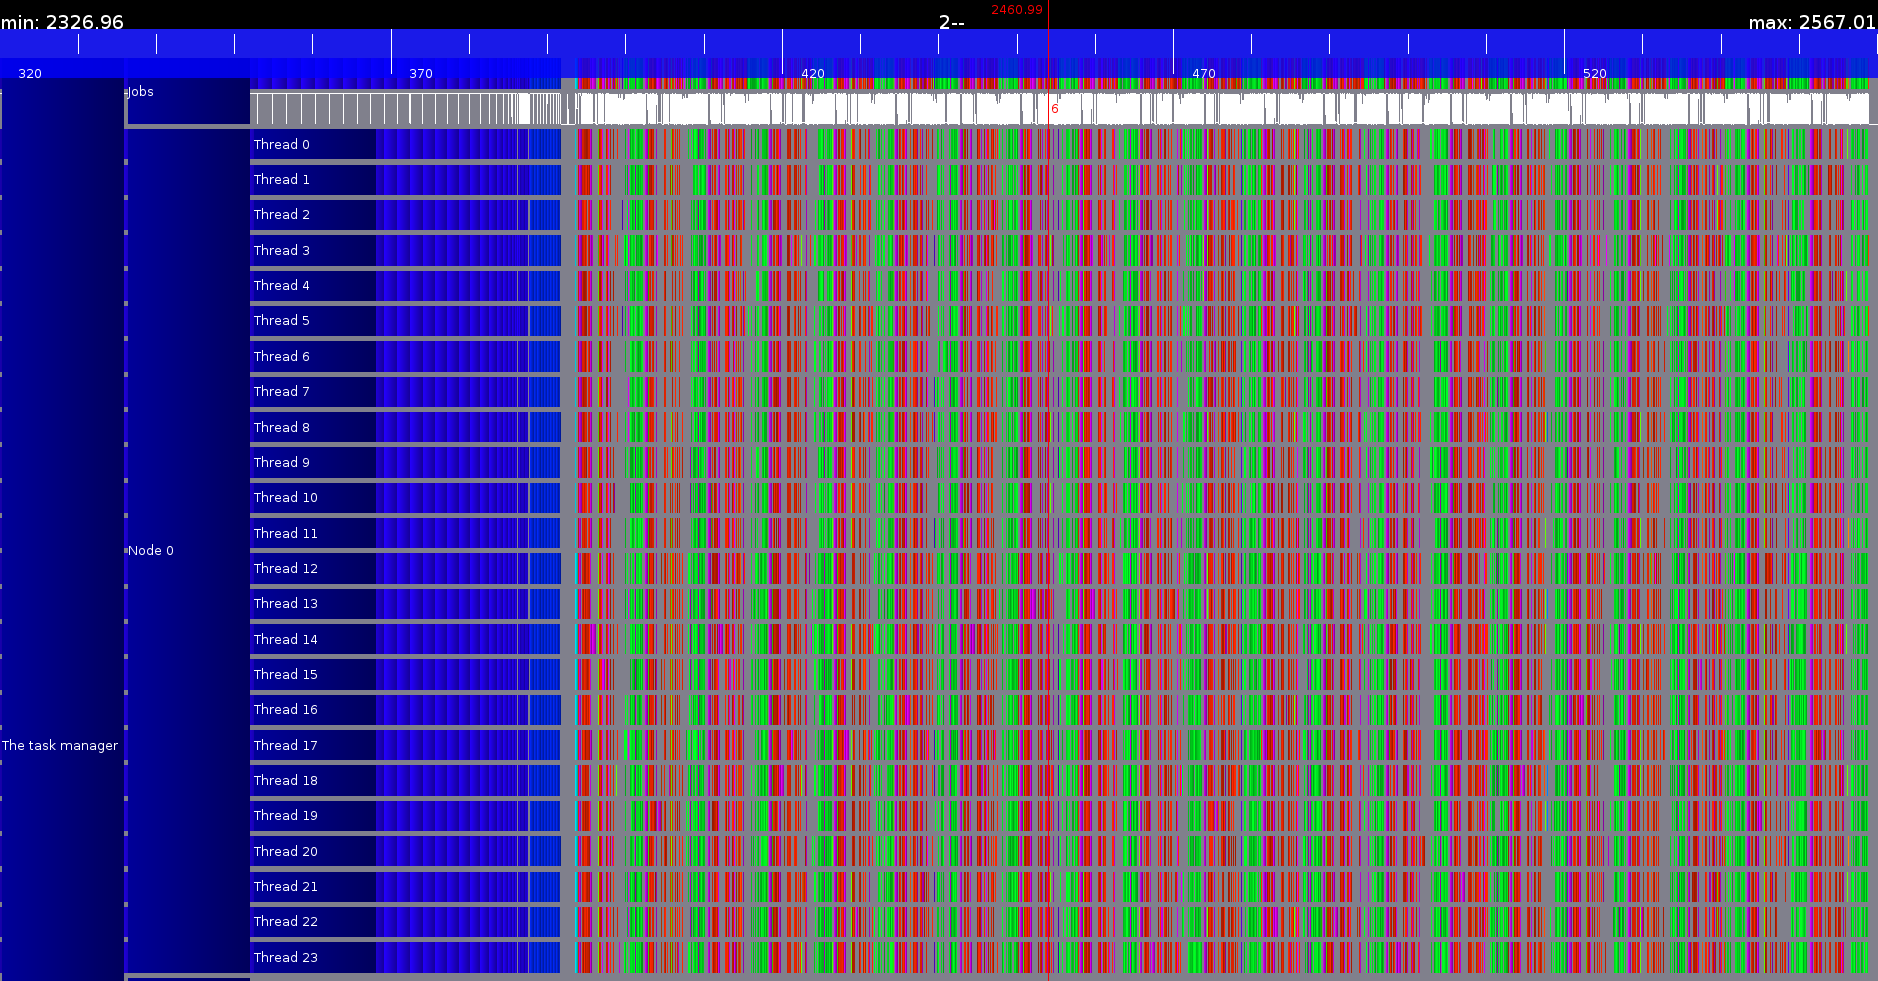
\includegraphics[width=1\linewidth]{iterations_trace.png}
\end{frame}


\end{document}

